\chapter{СУДАЛГААНЫ АРГА ЗҮЙ}

\section{Системийн ерөнхий тойм}
\subsection{Use Case Diagram}

Системийн хэрэглэгчийн харилцан үйлдлийг Use Case диаграммаар харуулав:

\begin{figure}[H]
\centering
\begin{tikzpicture}[
    scale=1.0, transform shape,
    usecase/.style={ellipse, draw=black, thick, minimum width=3.5cm, minimum height=1.2cm, align=center, font=\small},
    system/.style={rectangle, draw=black, dashed, thick, minimum width=9cm, minimum height=13cm},
    arrow/.style={-, thick}
]
    % System boundary
    \node[system, label={[font=\large\bfseries]above:FOREX Signal System}] (sys) at (5,-4) {};
    
    % Actor - Trader (left)
    \draw[thick] (-1.5,0) circle (0.3);
    \draw[thick] (-1.5,-0.3) -- (-1.5,-1);
    \draw[thick] (-1.5,-1) -- (-1.9,-1.8);
    \draw[thick] (-1.5,-1) -- (-1.1,-1.8);
    \draw[thick] (-1.9,-0.5) -- (-1.1,-0.5);
    \node[font=\small] at (-1.5,-2.2) {Арилжаачин};
    
    % Actor - Admin (bottom left)
    \draw[thick] (-1.5,-8) circle (0.3);
    \draw[thick] (-1.5,-8.3) -- (-1.5,-9);
    \draw[thick] (-1.5,-9) -- (-1.9,-9.8);
    \draw[thick] (-1.5,-9) -- (-1.1,-9.8);
    \draw[thick] (-1.9,-8.5) -- (-1.1,-8.5);
    \node[font=\small] at (-1.5,-10.2) {Админ};
    
    % Use cases - centered in system (swapped uc4 and uc5)
    \node[usecase] (uc1) at (5,1) {Дохио хүлээн авах};
    \node[usecase] (uc2) at (5,-1) {Таамаглал харах};
    \node[usecase] (uc3) at (5,-3) {Түүх харах};
    \node[usecase] (uc4) at (5,-5) {Мэдэгдэл авах};
    \node[usecase] (uc5) at (5,-7) {Тохиргоо хийх};
    \node[usecase] (uc6) at (5,-9) {Загвар сургах};
    
    % Connections from Trader to use cases
    \draw[arrow] (-1,-0.5) -- (uc1.west);
    \draw[arrow] (-1,-0.7) -- (uc2.west);
    \draw[arrow] (-1,-0.9) -- (uc3.west);
    \draw[arrow] (-1,-1.1) -- (uc4.west);
    \draw[arrow] (-1,-1.3) -- (uc5.west);
    
    % Connections from Admin to use cases
    \draw[arrow] (-1,-8.5) -- (uc5.west);
    \draw[arrow] (-1,-8.7) -- (uc6.west);
\end{tikzpicture}
\caption{Use Case Diagram}
\label{fig:usecase_diagram}
\end{figure}

\clearpage
\subsection{System Flow Diagram}

Системийн ажиллагааны үндсэн урсгалыг доорх диаграммаар харуулав:

\begin{figure}[H]
\centering
\begin{tikzpicture}[
    node distance=0.8cm and 1cm,
    auto,
    >=Stealth,
    font=\small,
    % Define styles with shadows and rounded corners
    base/.style={
        draw, thick, rounded corners, align=center,
        drop shadow, minimum height=1.0cm, minimum width=3cm
    },
    startstop/.style={
        base, rectangle, rounded corners=15pt,
        draw=red!80!black, fill=red!10
    },
    process/.style={
        base, rectangle,
        draw=blue!80!black, fill=blue!10
    },
    decision/.style={
        base, diamond, aspect=2.5,
        draw=orange!80!black, fill=orange!10, inner sep=0pt, font=\small\linespread{0.9}\selectfont
    },
    io/.style={
        base, trapezium, trapezium left angle=70, trapezium right angle=110,
        draw=green!80!black, fill=green!10
    },
    line/.style={draw, thick, ->, rounded corners=5pt}
]
    % Nodes
    \node (start) [startstop] {Эхлэх};
    \node (fetch) [io, below=of start] {Twelve Data API-аас\\бодит өгөгдөл татах};
    \node (validate) [decision, below=of fetch] {Өгөгдөл\\хүчинтэй?};
    \node (cache) [process, right=2.0cm of validate] {Cache-аас\\өгөгдөл авах};
    \node (features) [process, below=of validate] {Technical Indicators\\(Time, Trend, Volatility)};
    \node (predict) [process, below=of features] {Ensemble Model\\(XGBoost, LightGBM, CatBoost)};
    \node (conf) [decision, below=of predict] {Confidence $\geq$ Босго};
    
    % Branches
    \node (buy) [io, below left=0.5cm and 1cm of conf] {BUY дохио\\үүсгэх};
    \node (hold) [io, below right=0.5cm and 1cm of conf] {HOLD төлөв\\буцаах};
    
    \node (sltp) [process, below=of buy] {Динамик SL/TP\\(ATR-д суурилсан)};
    \node (db) [process, below=of sltp] {MongoDB-д\\хадгалах};
    
    % Convergence point for response
    \node (send) [io] at (conf |- db) [yshift=-1.5cm] {API хариу\\илгээх};
    \node (end) [startstop, below=of send] {Дуусах};
    
    % Paths
    \path [line] (start) -- (fetch);
    \path [line] (fetch) -- (validate);
    \path [line] (validate) -- node [pos=0.4] {Үгүй} (cache);
    \path [line] (cache) |- (features);
    \path [line] (validate) -- node [pos=0.4] {Тийм} (features);
    \path [line] (features) -- (predict);
    \path [line] (predict) -- (conf);
    
    % Decision paths
    \path [line] (conf) -| node [near start, above] {Тийм} (buy);
    \path [line] (conf) -| node [near start, above] {Үгүй} (hold);
    
    \path [line] (buy) -- (sltp);
    \path [line] (sltp) -- (db);
    
    % Connect to send
    \draw [line] (db) |- (send);
    \draw [line] (hold) |- (send);
    
    \path [line] (send) -- (end);

\end{tikzpicture}
\caption{Дохио үүсгэх системийн Flow Diagram}
\label{fig:flow_diagram}
\end{figure}

\subsection{Үйл ажиллагааны (Activity) диаграмм - Дохио авах үйлдэл}

Хэрэглэгч дохио авах үйлдлийн Үйл ажиллагааны (Activity) диаграмм:

\begin{figure}[H]
\centering
\begin{tikzpicture}[
    scale=0.85, transform shape,
    node distance=0.8cm,
    initial/.style={circle, draw=black, fill=black, minimum size=0.4cm},
    final/.style={circle, draw=black, thick, fill=white, minimum size=0.5cm, path picture={\fill[black] (path picture bounding box.center) circle (0.15cm);}},
    action/.style={rectangle, rounded corners=8pt, draw=black, thick, minimum width=2.4cm, minimum height=0.8cm, align=center, font=\small},
    decision/.style={diamond, draw=black, thick, fill=yellow!30, minimum width=1.4cm, minimum height=0.8cm, aspect=1.8, align=center, font=\small},
    mergepoint/.style={circle, draw=black, fill=black, minimum size=0.08cm, inner sep=0pt},
    arrow/.style={->, >=stealth, thick},
    line/.style={-, thick}
]
    % Swimlanes - Backend API wider (7cm)
    \node[rectangle, draw=black, thick, minimum width=3.5cm, minimum height=13cm, fill=blue!8] (s1) at (0,0) {};
    \node[rectangle, draw=black, thick, minimum width=7cm, minimum height=13cm, fill=green!8] (s2) at (5.5,0) {};
    \node[rectangle, draw=black, thick, minimum width=3.5cm, minimum height=13cm, fill=orange!8] (s3) at (11,0) {};
    
    % Swimlane labels - moved higher
    \node[font=\small\bfseries] at (0,6.8) {Mobile App};
    \node[font=\small\bfseries] at (5.5,6.8) {Backend Server};
    \node[font=\small\bfseries] at (11,6.8) {ML Model};
    
    % Mobile App actions
    \node[initial] (start) at (0,5.3) {};
    \node[action, fill=blue!15] (open) at (0,4.2) {Апп нээх};
    \node[action, fill=blue!15] (request) at (0,2.5) {Request Signal};
    \node[action, fill=blue!15] (display) at (0,-4.5) {Display\\Signal};
    \node[final] (end) at (0,-5.8) {};
    
    % Backend actions
    \node[action, fill=green!15] (fetch) at (4,2.5) {Fetch\\Data};
    \node[decision] (check) at (4,0.5) {Cache?};
    \node[action, fill=green!15] (api) at (7.2,0.5) {API Call};
    \node[mergepoint] (merge) at (5.5,-1.2) {};
    \node[action, fill=green!15] (process) at (5.5,-2.5) {Data\\Processing};
    \node[action, fill=green!15] (response) at (5.5,-4.5) {Send\\Response};
    
    % ML actions
    \node[action, fill=orange!15] (features) at (11,-2.5) {Feature\\Calculation};
    \node[action, fill=orange!15] (predict) at (11,-4.5) {Model\\Prediction};
    
    % Arrows - Mobile App
    \draw[arrow] (start) -- (open);
    \draw[arrow] (open) -- (request);
    
    % Arrow - Mobile to Backend
    \draw[arrow] (request.east) -- (fetch.west);
    
    % Arrow - fetch to check
    \draw[arrow] (fetch) -- (check);
    
    % Arrow - Cache? No -> API (with visible label)
    \draw[arrow] (check.east) -- node[above, font=\scriptsize] {Үгүй} (api.west);
    
    % Arrow - API -> merge point (down then left - no arrow head)
    \draw[line] (api.south) -- (7.2,-1.2) -- (merge);
    
    % Arrow - Cache? Yes -> merge point (down then right - no arrow head)
    \draw[line] (check.south) -- node[left, font=\scriptsize] {Тийм} (4,-1.2) -- (merge);
    
    % Arrow - merge point to process (SINGLE arrow)
    \draw[arrow] (merge) -- (process.north);
    
    % Arrow - process to features
    \draw[arrow] (process.east) -- (features.west);
    
    % Arrow - features to predict
    \draw[arrow] (features) -- (predict);
    
    % Arrow - predict to response (left then down - 90 degree)
    \draw[arrow] (predict.west) -- (9.5,-4.5) -- (response.east);
    
    % Arrow - response to display
    \draw[arrow] (response.west) -- (display.east);
    
    % Arrow - display to end
    \draw[arrow] (display) -- (end);
\end{tikzpicture}
\caption{Activity Diagram - Signal Fetching}
\label{fig:activity_diagram}
\end{figure}



\subsection{System Architecture Diagram}

Системийн бүрэлдэхүүн хэсгүүдийн харилцан холболтыг давхаргат архитектураар харуулав:

\begin{figure}[H]
\centering
\begin{tikzpicture}[scale=0.9, transform shape,
    box/.style={rectangle, draw=#1!70, line width=1pt, fill=#1!12, rounded corners=3pt, minimum height=1cm, align=center, font=\sffamily\small, drop shadow={shadow xshift=1pt, shadow yshift=-1pt, opacity=0.3}},
    layer/.style={rectangle, draw=#1!40, fill=#1!4, rounded corners=5pt, line width=0.8pt},
    db/.style={cylinder, draw=orange!70, fill=orange!12, shape border rotate=90, aspect=0.3, minimum height=0.9cm, minimum width=1.4cm, font=\sffamily\footnotesize, drop shadow={shadow xshift=1pt, shadow yshift=-1pt, opacity=0.3}},
    myarrow/.style={-{Stealth[length=3mm, width=2mm]}, line width=1pt, #1},
    mydarrow/.style={{Stealth[length=3mm, width=2mm]}-{Stealth[length=3mm, width=2mm]}, line width=1pt, #1},
    layerlabel/.style={font=\small\bfseries, align=center, anchor=north, yshift=-3pt}
]
    % === LAYERS ===
    % Layer 1: Application - Left
    \node[layer=violet, minimum width=3.2cm, minimum height=4.5cm] (L1) at (0,0) {};
    \node[layerlabel, text=violet!60!black] at (L1.north) {Client\\Side};
    
    % Layer 2: Backend - Middle Left
    \node[layer=blue, minimum width=3.2cm, minimum height=4.5cm] (L2) at (4.5,0) {};
    \node[layerlabel, text=blue!60!black] at (L2.north) {Server\\Side};
    
    % Layer 3: ML - Top Right
    \node[layer=green!60!black, minimum width=8.5cm, minimum height=2.8cm] (L3) at (13.0,1.6) {};
    \node[layerlabel, text=green!50!black] at (L3.north) {Machine Learning Models};
    
    % Layer 4: Data - Bottom Right
    \node[layer=orange, minimum width=8.5cm, minimum height=2.8cm] (L4) at (13.0,-1.8) {};
    \node[layerlabel, text=orange!60!black] at (L4.north) {Data Layer};
    
    % === COMPONENTS ===
    \node[box=violet, minimum width=2.6cm, minimum height=1.3cm] (app) at (0,-0.2) {Mobile App\\\scriptsize Expo + React Native};
    \node[box=blue, minimum width=2.6cm, minimum height=1.3cm] (api) at (4.5,-0.2) {Flask API\\\scriptsize Waitress WSGI};
    
    % ML Models
    \node[box=green!70!black, minimum width=1.8cm] (xgb) at (10.5,1.5) {\footnotesize XGB×3};
    \node[box=yellow!70!black, minimum width=1.8cm] (lgb) at (13.0,1.5) {\footnotesize LGB×2};
    \node[box=orange!70!black, minimum width=1.8cm] (cat) at (15.5,1.5) {\footnotesize CAT×2};
    
    % Data Components
    \node[db] (mongo) at (10.5,-2.1) {MongoDB};
    \node[box=cyan, minimum width=2.2cm] (twelve) at (15.0,-2.1) {\footnotesize Twelve Data};
    
    % === ARROWS ===
    % App <-> API
    \draw[mydarrow=violet!70] (app.east) -- (api.west);
    \node[font=\sffamily\scriptsize, fill=white, inner sep=1pt, text=violet!70, align=center] at (2.25,-0.2) {REST\\API};
    
    % API -> ML
    \draw[myarrow=blue!70] (api.east) -- ++(1.8,0) |- (L3.west) node[pos=0.2, above, font=\sffamily\scriptsize, fill=white, inner sep=1pt, align=center] {Request\\Prediction};
    
    % API <-> Data
    \draw[mydarrow=orange!70] (api.east) -- ++(1.8,0) |- (L4.west) node[pos=0.2, below, font=\sffamily\scriptsize, fill=white, inner sep=1pt] {Signal};
    
    % Data Flow
    \draw[myarrow=cyan!70] (twelve.west) -- (mongo.east) node[midway, above, font=\sffamily\scriptsize, text=cyan!80!black] {Real-time Price};
    
    % ML Ensemble Label
    \node[font=\sffamily\scriptsize\itshape, green!40!black] at (13.0,0.5) {Hybrid Ensemble (7 models)};

\end{tikzpicture}
\caption{System Architecture Diagram}
\label{fig:system_architecture}
\end{figure}

\subsection{Sequence Diagram - API Call}

API дуудлагын дарааллын диаграмм:

\begin{figure}[H]
\centering
\begin{tikzpicture}[scale=0.9, transform shape,
    actor/.style={rectangle, draw=black, fill=yellow!20, minimum width=2.2cm, minimum height=0.7cm, font=\sffamily\small\bfseries},
    msg/.style={-{Stealth[length=2.5mm]}, thick},
    ret/.style={{Stealth[length=2.5mm]}-, thick},
    lbl/.style={font=\sffamily\scriptsize, fill=white, inner sep=1pt}
]
    % === ACTORS ===
    \node[actor] (user) at (0,0) {Хэрэглэгч};
    \node[actor] (app) at (3.5,0) {Mobile App};
    \node[actor] (api) at (7,0) {Backend Server};
    \node[actor] (ml) at (10.5,0) {ML Model};
    \node[actor] (data) at (14,0) {Twelve Data};
    
    % === LIFELINES ===
    \draw[thick] (0,-0.5) -- (0,-9.5);
    \draw[thick] (3.5,-0.5) -- (3.5,-9.5);
    \draw[thick] (7,-0.5) -- (7,-9.5);
    \draw[thick] (10.5,-0.5) -- (10.5,-9.5);
    \draw[thick] (14,-0.5) -- (14,-9.5);
    
    % === ACTIVATION BOXES ===
    \fill[yellow!30] (3.35,-1.2) rectangle (3.65,-8.3);
    \fill[green!20] (6.85,-2.2) rectangle (7.15,-7.3);
    \fill[orange!20] (10.35,-5.2) rectangle (10.65,-6.3);
    \fill[cyan!20] (13.85,-3.2) rectangle (14.15,-4.3);
    
    % === MESSAGES ===
    % 1. Апп нээх
    \draw[msg] (0,-1.5) -- (3.35,-1.5);
    \node[lbl] at (1.75,-1.2) {1. Апп нээх};
    
    % 2. Дохио хүсэх
    \draw[msg] (3.65,-2.5) -- (6.85,-2.5);
    \node[lbl] at (5.25,-2.2) {2. Request Signal};
    
    % 3. Өгөгдөл татах
    \draw[msg] (7.15,-3.5) -- (13.85,-3.5);
    \node[lbl] at (10.5,-3.2) {3. Fetch Data};
    
    % 4. OHLCV өгөгдөл
    \draw[ret] (7.15,-4.3) -- (13.85,-4.3);
    \node[lbl] at (10.5,-4) {4. OHLCV Data};
    
    % 5. Таамаглал хүсэх
    \draw[msg] (7.15,-5.5) -- (10.35,-5.5);
    \node[lbl] at (8.75,-5.2) {5. Request Prediction};
    
    % 6. Таамаглал
    \draw[ret] (7.15,-6.3) -- (10.35,-6.3);
    \node[lbl] at (8.75,-6) {6. Prediction};
    
    % 7. Дохио илгээх
    \draw[ret] (3.65,-7.3) -- (6.85,-7.3);
    \node[lbl] at (5.25,-7) {7. Send Signal};
    
    % 8. Таамаглал хүлээн авах
    \draw[ret] (0,-8.3) -- (3.35,-8.3);
    \node[lbl] at (1.75,-8) {8. Receive Prediction};

\end{tikzpicture}
\caption{Sequence Diagram - API Call}
\label{fig:sequence_diagram}
\end{figure}

\section{Data Description}

\subsection{Data Source}

Энэхүү судалгаанд EUR/USD валютын хосын 1 минутын интервалтай түүхэн өгөгдлийг ашигласан. Өгөгдлийг Twelve Data API үйлчилгээнээс татан авсан бөгөөд дараах талбаруудыг агуулна:

\begin{itemize}
    \item \textbf{timestamp} - Timestamp (UTC)
    \item \textbf{open} - Open Price
    \item \textbf{high} - High Price
    \item \textbf{low} - Low Price
    \item \textbf{close} - Close Price
    \item \textbf{volume} - Volume
\end{itemize}

\subsection{Data Time Range}

\begin{table}[H]
\centering
\caption{Data Time Range}
\begin{tabular}{|l|l|l|r|}
\hline
\textbf{Dataset} & \textbf{Start Date} & \textbf{End Date} & \textbf{Rows} \\
\hline
Train Set & 2019-12-31 & 2024-12-30 & 1,859,492 \\
\hline
Test Set & 2024-12-31 & 2025-10-17 & 296,778 \\
\hline
\end{tabular}
\label{tab:data_range}
\end{table}

\subsection{Өгөгдлийн чанарын хяналт}

Өгөгдлийн чанарыг дараах алхмуудаар шалгаж, засварласан:

\begin{enumerate}
    \item \textbf{Давхардсан бичлэг шалгах:} Timestamp давхардсан бичлэгүүдийг устгах
    \item \textbf{Дутуу утга нөхөх:} Forward fill аргаар дутуу үнийн утгуудыг нөхөх
    \item \textbf{Аномали илрүүлэх:} Хэвийн бус үнийн өөрчлөлтүүдийг шалгах
\end{enumerate}

\section{Шинж чанар инженерчлэл}

Энэхүү судалгаанд суурь үзүүлэлтүүд дээр шинээр хосолсон шинж чанаруудыг (Hybrid Features) нэмж ашигласан.

\subsection{Features Summary}

Нийт 32 Technical Indicator-ийг дараах категориудаар бүлэглэв:

\begin{figure}[H]
\centering
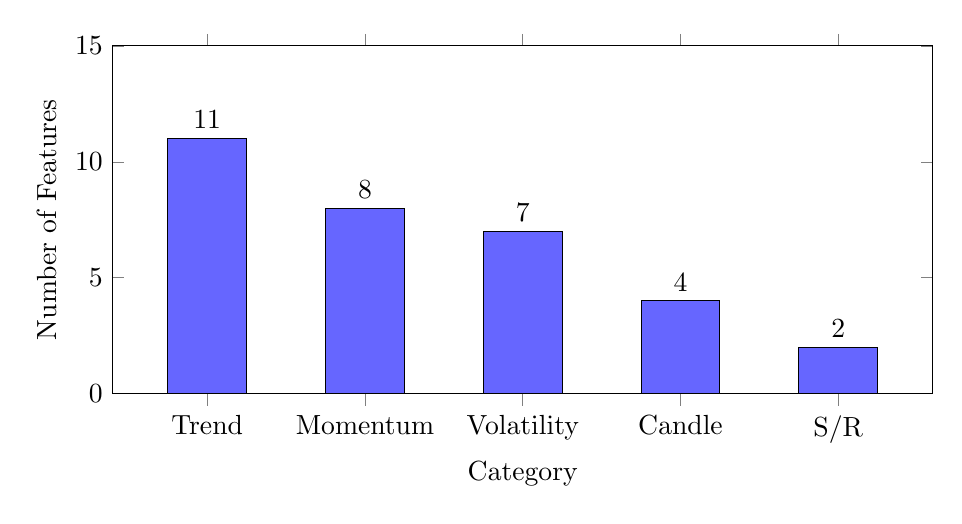
\begin{tikzpicture}
\begin{axis}[
    ybar,
    width=12cm,
    height=6cm,
    xlabel={Category},
    ylabel={Number of Features},
    symbolic x coords={Trend, Momentum, Volatility, Candle, S/R},
    xtick=data,
    nodes near coords,
    bar width=1cm,
    ymin=0,
    ymax=15,
    enlarge x limits=0.15,
]
\addplot[fill=blue!60] coordinates {
    (Trend, 11)
    (Momentum, 8)
    (Volatility, 7)
    (Candle, 4)
    (S/R, 2)
};
\end{axis}
\end{tikzpicture}
\caption{Number of Selected Features per Category}
\label{fig:feature_bar}
\end{figure}

\begin{itemize}
    \item \textbf{Trend Indicators (11):} SMA (5, 10, 20, 50), EMA (5, 20), ADX, Trend Score, Price vs MA
    \item \textbf{Momentum Indicators (8):} RSI (14), MACD, CCI, Williams \%R, Momentum Score, RSI Zone
    \item \textbf{Volatility Indicators (7):} ATR (14), Bollinger Bands (width, position), Volatility State, Breakout
    \item \textbf{Candle Patterns (4):} Body size, Wick ratio, Bullish/Bearish, Candle Streak
    \item \textbf{Support/Resistance (2):} Dist to High/Low (20 period)
\end{itemize}

\subsection{Core Features}

\subsubsection{Moving Averages}

Энгийн хөдөлгөөнт дундаж (SMA) ба экспоненциал хөдөлгөөнт дундаж (EMA)-ийг 6 өөр хугацаанд (5, 10, 20, 50, 100, 200) тооцоолсон.

\subsubsection{MA Crossover Signals}

Хөдөлгөөнт дундажийн огтлолцлыг BUY дохионы шинж чанар болгон ашигласан:

\begin{itemize}
    \item \textbf{sma\_5\_20\_cross} - if SMA(5) > SMA(20) then 1
    \item \textbf{sma\_20\_50\_cross} - if SMA(20) > SMA(50) then 1
    \item \textbf{ema\_10\_50\_cross} - if EMA(10) > EMA(50) then 1
    \item \textbf{golden\_cross} - if SMA(50) > SMA(200) then 1 (Golden Cross)
\end{itemize}

\subsection{Hybrid New Features}

Hybrid Ensemble загварын нарийвчлалыг нэмэгдүүлэхийн тулд дараах 10 шинэ бүлэг шинж чанарыг нэмсэн:

\begin{enumerate}
    \item \textbf{Trend Strength Score (0-5):} EMA огтлолцлууд болон ADX дээр суурилсан чиг хандлагын хүч.
    \item \textbf{Momentum Alignment:} RSI, MACD, CCI, Williams \%R зэрэг моментум индикаторуудын давхцал.
    \item \textbf{Volatility State:} Volatility SMA-тай харьцуулсан зах зээлийн тогтворгүй байдлын төлөв (High, Low, Normal).
    \item \textbf{Price Action Patterns:} Лааны биеийн харьцаа, wick-ийн урт зэрэг price action мэдээлэл.
    \item \textbf{Bullish Patterns:} Өсөлтийн лааны дараалал (bullish streak).
    \item \textbf{Support/Resistance Proximity:} 20-period High/Low цэгүүдтэй үнийн ойролцоо байдал.
    \item \textbf{Multi-timeframe Momentum:} RSI-ийн богино болон урт хугацааны дунджийн зөрүү.
    \item \textbf{Breakout Detection:} Bollinger Bands-ийн дээд/доод хязгаарыг давсан эсэх.
    \item \textbf{Price Momentum:} 5, 10, 20 минутын өмнөх үнэтэй харьцуулсан өөрчлөлт (ATR-аар жинлэсэн).
    \item \textbf{Session Quality:} London/NY session overlap үеийг онцолсон feature.
\end{enumerate}

\subsection{Momentum Indicators}

\subsubsection{RSI (Relative Strength Index)}

RSI-ийг 7, 14, 21 хугацаанд тооцоолсон:

\begin{equation}
RSI = 100 - \frac{100}{1 + RS}
\end{equation}

Энд $RS = \frac{\text{Average Gain}}{\text{Average Loss}}$

RSI Zones:
\begin{itemize}
    \item \textbf{rsi\_oversold} - if RSI(14) < 30 then 1 (Oversold)
    \item \textbf{rsi\_bullish} - if 50 < RSI(14) < 70 then 1 (Bullish Zone)
\end{itemize}

\subsubsection{MACD (Moving Average Convergence Divergence)}

\begin{align}
MACD &= EMA_{12} - EMA_{26} \\
Signal &= EMA_9(MACD) \\
Histogram &= MACD - Signal
\end{align}

MACD Signals:
\begin{itemize}
    \item \textbf{macd\_cross} - if MACD > Signal then 1
    \item \textbf{macd\_bullish} - if MACD > Signal and Histogram > 0 then 1
\end{itemize}

\subsubsection{Stochastic Oscillator}

\begin{equation}
\%K = \frac{C - L_{14}}{H_{14} - L_{14}} \times 100
\end{equation}

Энд $L_{14}$ ба $H_{14}$ нь 14 хугацааны хамгийн бага ба өндөр үнэ.

\subsubsection{ROC (Rate of Change)}

\begin{equation}
ROC_n = \frac{C_t - C_{t-n}}{C_{t-n}} \times 100
\end{equation}

\subsection{Volatility Indicators}

\subsubsection{ATR (Average True Range)}

ATR is crucial for calculating Stop Loss and Take Profit:

\begin{equation}
TR = max(H - L, |H - C_{prev}|, |L - C_{prev}|)
\end{equation}

\begin{equation}
ATR_{14} = SMA_{14}(TR)
\end{equation}

Converting ATR to pips:
\begin{equation}
ATR_{pips} = ATR_{14} \times 10000
\end{equation}

\subsubsection{Bollinger Bands}

\begin{align}
BB_{middle} &= SMA_{20} \\
BB_{upper} &= BB_{middle} + 2 \times \sigma_{20} \\
BB_{lower} &= BB_{middle} - 2 \times \sigma_{20}
\end{align}

Bollinger Bands Features:
\begin{itemize}
    \item \textbf{bb\_width} - Band Width (\%)
    \item \textbf{bb\_position} - Price Position (0-1)
    \item \textbf{bb\_squeeze} - Squeeze Detected (1)
\end{itemize}

\subsection{Candle Patterns}

Лааны биеийн хэмжээ, сүүдрийн урт зэргийг тооцоолж, bullish engulfing, hammer зэрэг загваруудыг илрүүлсэн.

\subsection{Support/Resistance}

Pivot Point системийг ашигласан:

\begin{align}
Pivot &= \frac{H_{prev} + L_{prev} + C_{prev}}{3} \\
R1 &= 2 \times Pivot - L_{prev} \\
S1 &= 2 \times Pivot - H_{prev} \\
R2 &= Pivot + (H_{prev} - L_{prev}) \\
S2 &= Pivot - (H_{prev} - L_{prev})
\end{align}

\subsection{Trend Strength}

Гурван хугацааны (богино, дунд, урт) чиг хандлагыг нэгтгэн trend\_alignment үзүүлэлтийг тооцоолсон. Бүх гурван хугацаа өсөлтийн чиглэлтэй бол strong\_uptrend = 1 гэж тодорхойлсон.

\subsection{BUY Score}

BUY дохионы хүчийг MACD, RSI, MA crossover, Golden Cross, чиг хандлага зэрэг индикаторуудын нийлбэр оноогоор тодорхойлсон.

\section{Target Variable}

\subsection{BUY-only Classification}

Энэхүү судалгаанд BUY дохиог таамаглахад анхаарал хандуулсан. Зорилтот хувьсагчийг дараах байдлаар тодорхойлсон:

\begin{itemize}
    \item \textbf{BUY (1):} Take Profit (TP) hit before Stop Loss (SL)
    \item \textbf{NOT\_BUY (0):} SL hit first or neither reached
\end{itemize}

\subsection{Parameters}

\begin{table}[H]
\centering
\caption{Target Variable Parameters}
\begin{tabular}{|l|l|l|}
\hline
\textbf{Parameter} & \textbf{Value} & \textbf{Description} \\
\hline
Forward periods & 60 bars & Within 1 hour \\
\hline
Take Profit & 20 pips & Profit Target \\
\hline
Stop Loss & 10 pips & Loss Limit \\
\hline
Risk:Reward & 1:2 & Risk/Reward Ratio \\
\hline
\end{tabular}
\label{tab:target_params}
\end{table}

\section{Data Split and Scaling}

\subsection{Splitting}

Санхүүгийн өгөгдөлд хугацааны дарааллыг хадгалах шаардлагатай тул temporal split ашигласан:

\begin{itemize}
    \item \textbf{Train Set:} 2019-12-31 - 2024-12-30 (1,859,492 rows)
    \item \textbf{Test Set:} 2024-12-31 - 2025-10-17 (296,778 rows)
\end{itemize}

\subsection{StandardScaler}

Бүх шинж чанаруудыг StandardScaler ашиглан scaled:

\begin{equation}
x_{scaled} = \frac{x - \mu}{\sigma}
\end{equation}

\section{Model Architecture}

\subsection{Proposed Hybrid Ensemble Method}

Энэхүү судалгаанд долоон машин сургалтын моделийн нэгдэл буюу ensemble аргыг ашигласан бөгөөд үүнийг ``Hybrid Ensemble System'' гэж нэрлэв. Гурван ялгаатай алгоритмын олон хувилбарыг нэгтгэснээр илүү найдвартай таамаглал гаргана:

\begin{enumerate}
    \item \textbf{XGBoost × 3} - Gradient Boosting Decision Trees (3 different hyperparameters)
    \item \textbf{LightGBM × 2} - Light Gradient Boosting Machine (2 different configs)
    \item \textbf{CatBoost × 2} - Categorical Boosting (2 different configs)
\end{enumerate}

\begin{figure}[H]
\centering
\begin{tikzpicture}[
    scale=0.9, transform shape,
    % Basic block styles
    block/.style={rectangle, draw=gray!80, line width=0.8pt, rounded corners=4pt, minimum width=2.2cm, minimum height=1cm, font=\sffamily\small, align=center, fill=white},
    % Input/System/Output styles
    feature/.style={block, fill=blue!10, minimum width=6cm, minimum height=1.2cm},
    system/.style={block, fill=cyan!15, minimum width=12cm, minimum height=1.2cm, rounded corners=6pt},
    ensemble/.style={block, fill=red!15, minimum width=8cm},
    output/.style={block, fill=purple!15, minimum width=4cm, font=\bfseries},
    % Group container style
    group_box/.style={rectangle, draw, line width=1pt, rounded corners=6pt, inner sep=10pt, align=center, fill opacity=0.1},
    % Inner model label style (simple textual boxes)
    inner_model/.style={rectangle, draw=gray!60, line width=0.5pt, rounded corners=2pt, minimum width=2.5cm, minimum height=0.7cm, font=\sffamily\footnotesize, align=center},
    % Connectors
    arrow/.style={-{Stealth[scale=1.0]}, thick, color=gray!70!black}
]

    % === LEVEL 1: INPUT ===
    \node[feature] (input) at (0,0) {Hybrid Features};

    % === LEVEL 2: GROUPS (Horizontal Layout of Groups) ===
    
    % --- LightGBM Group (Left) ---
    % 2 Models
    \node[group_box, draw=yellow!60!black, fill=yellow!50, minimum width=4cm, minimum height=4cm] (lgb_group) at (-5, -4) {};
    % Inside
    \node[inner_model, fill=yellow!15] at (-5, -3.2) {LightGBM-1};
    \node[inner_model, fill=yellow!15] at (-5, -4.5) {LightGBM-2};

    % --- XGBoost Group (Center) ---
    % 3 Models
    \node[group_box, draw=green!60!black, fill=green!50, minimum width=4cm, minimum height=5cm] (xgb_group) at (0, -4.5) {};
    % Inside
    \node[inner_model, fill=green!15] at (0, -3.2) {XGBoost-1};
    \node[inner_model, fill=green!15] at (0, -4.5) {XGBoost-2};
    \node[inner_model, fill=green!15] at (0, -5.8) {XGBoost-3};

    % --- CatBoost Group (Right) ---
    % 2 Models
    \node[group_box, draw=orange!60!black, fill=orange!50, minimum width=4cm, minimum height=4cm] (cat_group) at (5, -4) {};
    % Inside
    \node[inner_model, fill=orange!15] at (5, -3.2) {CatBoost-1};
    \node[inner_model, fill=orange!15] at (5, -4.5) {CatBoost-2};

    % === LEVEL 3: AGGREGATION ===
    % Position relative to the lowest group (XGBoost ends at -7 or so)
    \node[system] (agreement) at (0,-8.5) {Agreement Bonus System};

    % === LEVEL 4: ENSEMBLE ===
    \node[ensemble] (weighted) at (0,-10.0) {Weighted Ensemble + Bonus};

    % === LEVEL 5: OUTPUT ===
    \node[output] (final) at (0,-11.5) {BUY Confidence};

    % === CONNECTIONS ===
    
    % Input -> Groups (Top of containers)
    \draw[arrow] (input.south) -- +(0,-0.6) -| (lgb_group.north);
    \draw[arrow] (input.south) -- (xgb_group.north);
    \draw[arrow] (input.south) -- +(0,-0.6) -| (cat_group.north);

    % Groups (Bottom of containers) -> Agreement
    % Draw straight vertical lines from each group to the Agreement box directly below it
    \draw[arrow] (lgb_group.south) -- (lgb_group.south |- agreement.north);
    \draw[arrow] (xgb_group.south) -- (xgb_group.south |- agreement.north);
    \draw[arrow] (cat_group.south) -- (cat_group.south |- agreement.north);

    % Agreement flow
    \draw[arrow] (agreement.south) -- (weighted.north);
    \draw[arrow] (weighted.south) -- (final.north);

\end{tikzpicture}
\caption{Hybrid Ensemble Model Architecture (7 models)}
\label{fig:ensemble_arch}
\end{figure}

\subsection{XGBoost Models}

XGBoost (eXtreme Gradient Boosting) нь gradient boosting framework дээр суурилсан алгоритм юм. Энэхүү системд гурван өөр hyperparameter-тэй XGBoost загварыг ашигласан:

\begin{itemize}
    \item \textbf{XGB-1:} n\_estimators=500, max\_depth=6, learning\_rate=0.03
    \item \textbf{XGB-2:} n\_estimators=400, max\_depth=8, learning\_rate=0.05
    \item \textbf{XGB-3:} n\_estimators=300, max\_depth=5, learning\_rate=0.08
\end{itemize}

\subsection{LightGBM Models}

LightGBM нь Microsoft-ийн боловсруулсан хурдан gradient boosting framework юм:

\begin{itemize}
    \item \textbf{LGB-1:} n\_estimators=500, max\_depth=6, learning\_rate=0.03
    \item \textbf{LGB-2:} n\_estimators=400, max\_depth=8, learning\_rate=0.05
\end{itemize}

\subsection{CatBoost Models}

CatBoost нь Yandex-ийн боловсруулсан, categorical feature-тэй сайн ажилладаг алгоритм:

\begin{itemize}
    \item \textbf{CAT-1:} iterations=500, depth=6, learning\_rate=0.03
    \item \textbf{CAT-2:} iterations=400, depth=8, learning\_rate=0.05
\end{itemize}

\subsection{Agreement Bonus System}

Agreement Bonus системийн гол шинэлэг тал бол загваруудын ``зөвшилцөл''-д суурилсан нэмэлт оноо юм. Бүх загварууд ижил таамаглал гаргах тусам итгэлцүүр нэмэгддэг:

\begin{table}[H]
\centering
\caption{Agreement Bonus System}
\begin{tabular}{|c|c|l|}
\hline
\textbf{Agreement} & \textbf{Bonus Score} & \textbf{Description} \\
\hline
7/7 models & +7\% & All same prediction \\
\hline
6/7 models & +4\% & All but one same \\
\hline
5/7 models & +2\% & Majority same \\
\hline
\end{tabular}
\label{tab:agreement_bonus}
\end{table}

\subsection{Weighted Ensemble}

Долоон загварын магадлалыг жинлэгдсэн дунджаар нэгтгэж, agreement bonus нэмнэ:

\begin{equation}
P_{base} = \sum_{i=1}^{7} w_i \cdot P_i(BUY)
\end{equation}

\begin{equation}
P_{final} = P_{base} + \text{Agreement Bonus}
\end{equation}

Энд $w_i$ нь загвар бүрийн жин (нийлбэр нь 1.0)

\subsection{Hyperparameters}

\begin{table}[H]
\centering
\caption{Ensemble Model Hyperparameters}
\begin{tabular}{|l|l|l|l|l|}
\hline
\textbf{Parameter} & \textbf{XGB-1} & \textbf{XGB-2/LGB-1} & \textbf{LGB-2} & \textbf{CatBoost} \\
\hline
n\_estimators & 500 & 400 & 400 & 400-500 \\
\hline
max\_depth & 6 & 8 & 8 & 6-8 \\
\hline
learning\_rate & 0.03 & 0.05 & 0.05 & 0.03-0.05 \\
\hline
subsample & 0.8 & 0.8 & 0.8 & 0.8 \\
\hline
colsample & 0.8 & 0.8 & 0.8 & 0.8 \\
\hline
\end{tabular}
\label{tab:hyperparams}
\end{table}

\section{Confidence Threshold}

Системийн итгэлцүүрийн босго нь дохиог үүсгэх эсэхийг тодорхойлно:

\begin{itemize}
    \item $P_{BUY} \geq 85\%$: Generate BUY signal (96.9\% accuracy)
    \item $P_{BUY} \geq 80\%$: BUY signal (71.8\% accuracy)
    \item $P_{BUY} < 80\%$: HOLD (wait)
\end{itemize}

85\% босго нь хамгийн оновчтой бөгөөд 96.9\% нарийвчлал (accuracy), өндөр ашигт ажиллагаатай байна.

\section{Dynamic SL/TP Calculation}

Stop Loss ба Take Profit-ийг ATR дээр суурилан динамикаар тооцоолно:

\begin{align}
SL_{pips} &= ATR_{pips} \times 1.5 \\
TP_{pips} &= ATR_{pips} \times 2.5
\end{align}

Хамгийн бага утгууд:
\begin{itemize}
    \item $SL_{min} = 8$ pips
    \item $TP_{min} = 12$ pips
\end{itemize}

\section{Backend API}

\subsection{Flask + Waitress}

Backend хэсэг нь Flask фреймворк ба Waitress WSGI сервер ашиглан хөгжүүлэгдсэн. /signal endpoint нь Twelve Data API-аас өгөгдөл авч, ML загваруудаар таамаглал хийж, JSON хэлбэрээр дохио буцаана.

\subsection{Twelve Data API}

Бодит цагийн болон түүхэн өгөгдлийг Twelve Data API-аас авдаг:

\begin{itemize}
    \item \textbf{Live rate:} \texttt{/price} endpoint
    \item \textbf{Historical data:} \texttt{/time\_series} endpoint
    \item \textbf{Cache TTL:} Live - 2 minutes, Historical - 5 minutes
    \item \textbf{Rate limit:} 1 request/minute (free tier)
\end{itemize}

\section{Mobile App Development}

\subsection{Technology Stack}

Системийн хэрэглэгчийн талыг React Native фреймворк ашиглан ``Cross-platform'' хэлбэрээр хөгжүүлсэн. Энэ нь нэг кодын баазаас Android болон iOS үйлдлийн системүүд дээр ажиллах боломжийг олгоно.

\begin{itemize}
    \item \textbf{Framework:} React Native (Expo SDK 51)
    \item \textbf{Language:} JavaScript (ES6+)
    \item \textbf{Navigation:} React Navigation (Stack \& Bottom Tabs)
    \item \textbf{State Management:} React Context API
    \item \textbf{Storage:} AsyncStorage (Local data \& Tokens)
    \item \textbf{Networking:} Axios (REST API client)
\end{itemize}

\subsection{Architecture and Structure}

Аппликейшн нь бүрэлдэхүүн хэсгүүдэд (Component-based architecture) суурилсан бүтэцтэй:

\begin{itemize}
    \item \textbf{Screens:} Үндсэн дэлгэцүүд (Home, Signal, Profile, Auth)
    \item \textbf{Components:} Дахин ашиглагдах UI хэсгүүд (Cards, Inputs, Buttons)
    \item \textbf{Context:} Глобал төлөв (Theme, Authentication)
    \item \textbf{Services:} API дуудлага ба логик
\end{itemize}

\subsection{Main App Features}

\subsubsection{1. Real-time Signal Dashboard}
SignalScreen нь Ensemble моделийн гаргасан таамаглалыг хэрэглэгчдэд ойлгомжтой байдлаар харуулна:
\begin{itemize}
    \item \textbf{Gauge Chart:} Итгэлцлийн хувийг (Confidence Score) графикаар харуулах
    \item \textbf{Signal Card:} BUY/SELL/HOLD дохио, Entry Price, Stop Loss, Take Profit утгууд
    \item \textbf{Market Info:} Валютын хосын spread, зах зээлийн төлөв (Closed/Open)
    \item \textbf{Pull-to-Refresh:} Дэлгэцийг доош татах үед шинэ сигнал татах
\end{itemize}

\subsubsection{2. AI Market Analysis}
Хэрэглэгч зөвхөн тоон утга харахаас гадна хиймэл оюун ухааны дүгнэлтийг унших боломжтой:
\begin{itemize}
    \item Техникийн индикаторуудын нэгдсэн дүгнэлт
    \item Эрсдэлийн түвшний зөвлөмж
    \item Зах зээлийн хандлагын тайлбар
\end{itemize}

\subsubsection{3. User Settings}
\begin{itemize}
    \item \textbf{Dark/Light Mode:} Системийн тохиргоо эсвэл хэрэглэгчийн сонголтоор солих
    \item \textbf{Confidence Threshold:} Хэрэглэгч өөрийн эрсдэлийн түвшинд тааруулан босго оноог (75\%, 80\%, 85\%) өөрчлөх боломж
\end{itemize}

\subsection{Security}

\begin{enumerate}
    \item \textbf{Token Storage:} Нэвтрэх token-ийг төхөөрөмж дээр шифрлэгдсэн хэлбэрээр хадгалах
    \item \textbf{Auto Logout:} Token хүчингүй болох үед автоматаар гаргах
    \item \textbf{Validation:} Бүртгүүлэх үед имэйл баталгаажуулалт, нууц үгийн нарийн шаардлага
\end{enumerate}

\subsection{API Integration}

Backend API-тай харилцахдаа RESTful зарчмыг баримтална:
\begin{itemize}
    \item \texttt{GET /signals/best} - Хамгийн сайн Ensemble загварын таамаглалыг авах
    \item \texttt{POST /auth/login} - Нэвтрэх, JWT token авах
    \item \texttt{POST /auth/register} - Шинэ хэрэглэгч бүртгэх
\end{itemize}

\section{MongoDB Database}

\subsection{Collections}

\begin{itemize}
    \item \textbf{users} - Хэрэглэгчийн мэдээлэл, нууц үг (bcrypt hash)
    \item \textbf{signals} - Хадгалагдсан дохионууд
    \item \textbf{verification\_codes} - Имэйл баталгаажуулалтын код (TTL: 10 мин)
\end{itemize}

\subsection{Authentication}

JWT (JSON Web Token) ашиглан хэрэглэгчийг баталгаажуулна:

\begin{itemize}
    \item \textbf{Token Validity}: 7 days
    \item \textbf{Algorithm}: HS256
    \item \textbf{Payload}: user\_id, email, exp (expiration)
    \item \textbf{Encryption}: SECRET\_KEY ашиглан encode хийнэ
\end{itemize}
